\documentclass[fleqn]{article}
\usepackage{amsmath}
\usepackage{amsfonts}
\usepackage{float}
\usepackage{pgfplots}
\usepackage{pgfplotstable}
\pgfplotsset{compat=1.17}

\title{Soluciones Estadística Descriptiva}
\author{Juan Rodriguez}

\begin{document}
	\maketitle
	\section{Solución Ejercicio 1}
	\begin{itemize}
		\item $\bar{x} = \frac{\sum_{i=1}^n x_i}{n} = \frac{7.1}{5} = 1.42$
		\item $\bar{y} = \frac{\sum_{i=1}^n y_i}{n} = \frac{131}{5} = 26.2$ 
		\item $s_x^{2} = \frac{\sum_{i=1}^n x_i^{2}}{n} - \bar{x}^{2} = \frac{15.565}{5} - 1.42^{2} = 1.1$ $s_x = 1.05$
		\item $s_y^{2} = \frac{\sum_{i=1}^n y_i^{2}}{n} - \bar{y}^{2} = \frac{5313}{5} - 26.2^{2} = 376.16$ $s_y = 19.4$
		\item $s_{xy} = \frac{\sum_{i=1}^n x_i y_i}{n} - \bar{x} \bar{y} = \frac{285.6}{5} - (1.42 \cdot 26.2) = 19.92$
	\end{itemize}
	a) Para saber si las variables están linealmente relacionadas, calculamos r
	\[
	r = \frac{s_{xy}}{s_x \cdot s_y} = \frac{19.92}{1.05 \cdot 19.4} = \boxed{0.98}
	\]
	\[
	R^2 = r^2 = (0.98)^{2} = \boxed{96.08\%}
	\]
	Interdependencia directa muy fuerte: la velocidad de reacción aumenta con la concentración de glucosa \\
	Los valores teóricos están muy cerca de los observados \\
	Las predicciones tienen una fiabilidad del 96.08\% y el ajuste es muy bueno \\
	Las dos rectas de regresión son casi coincidentes \\
	b) Nos piden predecir la concentración de glucosa a partir de una velocidad de 45 micromoles/minuto. Por lo tanto, usamos una recta de $X | Y$
	\[
	x - \bar{x} = \frac{s_{xy}}{s_y^{2}} (y - \bar{y}) \rightarrow x - 1.42 = 0.05(y - 26.2) \rightarrow x = 0.05y + 0.11
	\]
	\[
	x = 0.05(45) + 0.11 = 2.36
	\]
	La concentración de glucosa sera 2.36 milimoles/litro con una velocidad de 45 micromoles/minuto \\
	c) $b_yx = \frac{s_{xy}}{s_x^2} = \frac{19.92}{1.1} = 18.11$
	Por cada milimol/litro de glucogenosa, la velocidad de reacción aumenta 18.11 micromoles/minuto
	d)
	\[
	V_r = s_y^2 (1-r^2) = 376.16 \cdot (1-0.9608) = \boxed{14.9} 
	\]
	No quedan explicadas 14.9 unidades de varianza de la velocidad de reacción por la concentración de glucosa. Representan un 3.92\% de la variabilidad total \\
	f) $Q_1 = 10$, $Me = 18$, $Q_3 = 35$
	\begin{figure}[H]
		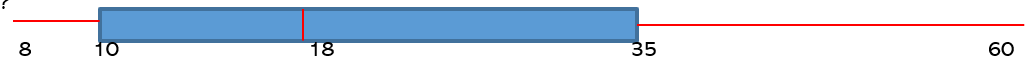
\includegraphics[width=0.9\textwidth]{boxplot.png}
	\end{figure}
	Vemos que presenta asimetría hacia la derecha ya que $Q_3 - Me > Me - Q_1$. Por lo que la media es mayor que la mediana. Además, se evidencia que hay mayor dispersión en los valores más altos (35 - 60)
	\section{Solución Ejercicio 2}
	\begin{itemize}
		\item $p(R) = 0.3$
		\item $p(N) = 0.5$
		\item $p(I) = 0.2$
		\item $p(D/R) = 0.01$
		\item $p(D/N) = 0.01$
		\item $p (D/I) = 0.015$
	\end{itemize}
	R - vuelos regionales; N - vuelos nacionales; I - vuelos internacionales; D - Reclamaciones
	a) Primero calculamos la probabilidad de internacional y no reclamación
	\[
	p(I \cap \bar{D}) = p(\bar{D}/I) \cdot p(I) = (1 - p(D/I)) \cdot p(I) = (1 - 0.015) \cdot 0.2 = 0.197
	\]
	Ahora definimos nuestra variable: X $\equiv$ número de clientes con destino internacional y no reclamación ~ $B(10, 0.197)$
	\[
	p(X \geq 2) = 1 - p(X < 2) = 1 - (p(X=0) + p(X=1)) = 1 - (\binom{10}{0}0.197^{0} \cdot 0.803^{10} + \binom{10}{1}0.197^{1} \cdot 0.803^{9}) = \boxed{0.615}
	\]
	b) Primero calculamos la probabilidad de D
	\[
	p(D) = p(D/R) \cdot p(R) + p(D/N) \cdot p(N) + p(D/I) \cdot p(I) = (0.3 \cdot 0.01) + (0.5 \cdot 0.01) + (0.2 \cdot 0.015) = 0.011 
	\]
	Ahora definimos nuestra variable: Y $\equiv$ número de contratos sin reclamación hasta que se produce la quinta reclamación ~ $BN(5;0.011)$
	\[
	p(Y = 35) = \binom{35 + 5 - 1}{35}0.011^{5} \cdot 0.989^{35} = \boxed{8.99 \cdot 10^{-6} \approx 0} 
	\]
	c) Conocemos la probabilidad de D condicionada por I - $p(D/I) = 0.015$. Sabiendo esto, definimos nuestra variable: T $\equiv$ número de contratos sin reclamación hasta que se produce la primera reclamación en un vuelo internacional ~ $G(0.015)$
	\[
	E[T] = \mu = \frac{0.985}{0.015} = 65.67 \approx 66 
	\]
	Entonces, el número medio de viajes contratados es $66+1=67$ viajes en total 
	\section{Solución Ejercicio 3}
	Definimos nuestra variable: X $\equiv$ ventas diarias en cientos de productos de un centro comercial \\
	a) Determinamos el valor de k para que f(x) sea una función de densidad
	\[
	\int_{1}^{3} k(x-1)(3-x)dx = 1 \rightarrow k\int_{1}^{3} (-x^2 +4x -3)dx = 1 \rightarrow k\frac{4}{3} = 1 \rightarrow \boxed{k = 3/4}
	\]
	b) La función de distribución es:
	\[
	F(x) = 
	\begin{cases}
		0 & \text{si } x < 1 \\
		\int_{1}^{x}\frac{3}{4}(t - 1)(3 - t) dt & \text{si } 1 \leq x \leq 3 \\
		1 & \text{si } x > 3
	\end{cases}
	\]
	c) Nos piden la probabilidad de que un día al azar venda más de 200 productos. Como los productos están en cientos, entonces $x = 2$
	\[
	P(X > 2) = 1 - p(X \leq 2) = 1 - F(2) = 1 - \int_{2}^{3}\frac{3}{4}(x - 1)(3 - x) dx = 1 - 0.5 = 0.5 
	\]
	Ahora definimos otra variable para la condición de que al menos un día de la semana se cumpla: T $\equiv$ número de días en que se vende más de 2 cientos de productos ~ $B(7;0.5)$
	\[
	p(T \geq 1) = 1 - p(T < 1) = 1 - p(T = 0) = 1 - \binom{7}{0} 0.5^0 \cdot 0.5^7 = \boxed{0.99}
	\]
	\section{Solución Ejercicio 4}
	Definimos nuestra variable: X $\equiv$ Tamaño de grano de aluminio ~ $N(96,14)$ \\
	a)
	\[
	p(X > 100) = 1 - p(X \leq 100) = 1 - p(\frac{X-96}{14} \leq \frac{100-96}{14}) = 1 - p(Z \leq 0.28) = 1 - 0.6103 = \boxed{0.38}
	\]
	b)
	\[
	p(50 \leq X \leq 80) = p(\frac{50-96}{14} \leq \frac{X-96}{14} \leq \frac{80-96}{14}) = p(-3.28 \leq Z \leq -1.14) = \boxed{0.126} 
	\]
	c) Nos piden hallar el 90\% central. Por lo tanto sabemos que es el area comprendida entre el percentil 5 y el percentil 95
	\[
	X_{5\%} = \mu + Z_{5\%} \cdot \sigma = 96 + (-1.645) \cdot 14 = 72.97
	\]
	\[
	X_{95\%} = \mu + Z_{95\%} \cdot \sigma = 96 + (1.645) \cdot 14 = 119.03
	\]
	Por lo tanto, el 90\% central esta en el intervalo $(72.97, 119.03)$
\end{document}